\section{Technical acknowledgements}
\paragraph{}
The following code presented was written using \emph{R}. The images from which the shapes were extracted were used as gray images. \ref{fig:gray-images}

\section{Loading data}
\paragraph{}
Images are loaded then converted to grayscale. Right now, we are not interested in their color, so they'll only be black and white.

\begin{lstlisting}[language=R, caption=Loading images in R]
    rdfReadGreyImage <- function (nom) {
        image <- readImage (paste('images/', nom, sep=''))
        if (length (dim (image)) == 2) {
            image
        } else {
            channel (image, 'red')
        }
    }
\end{lstlisting}

\begin{figure}[h]
    \centering
    
\includegraphics[scale=2.0]{rdf-carre-6.png}
    
\includegraphics[scale=2.0]{rdf-carre-10.png}
    
\includegraphics[scale=2.0]{rdf-carre-10-30deg.png}
    
\includegraphics[scale=2.0]{rdf-triangle-10-15deg.png}
    
\includegraphics[scale=2.0]{rdf-triangle-10-45deg.png}
    
\includegraphics[scale=2.0]{rdf-triangle-10-60deg.png}
    
\includegraphics[scale=2.0]{rdf-triangle-20.png}
    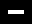
\includegraphics[scale=2.0]{rdf-rectangle-horizontal.png}
    
\includegraphics[scale=2.0]{rdf-rectangle-vertical.png}
    
\includegraphics[scale=2.0]{rdf-rectangle-diagonal.png}
    \caption{Shape images}
    \label{fig:gray-images}
\end{figure}

\clearpage

\section{Moments of a shape}
\subsection{Prerequisites}
\paragraph{}
We define the \emph{moment of a shape} as the following:
$$M_{ij} = \sum_{x}\sum_{y} x^{i} y^{j} A(x, y)$$
\paragraph{}
where $A(x, y)$ is the value of the pixel $(x, y)$ of the shape's image. One can easily observe that $M_{00}$ is equal to the number of pixels that are not black. We call that the \emph{surface} of the shape.

\begin{lstlisting}[language=R, caption=Calculating the moment of a shape]
    rdfMoment <- function (im, p, q) {
        x <- (1 : (dim (im)[1])) ^ p
        y <- (1 : (dim (im)[2])) ^ q
        as.numeric (rbind (x) %*% im %*% cbind (y))
        }
\end{lstlisting}

\paragraph{}
The \emph{barycenter} is defined as being the following:
$$(\bar{x}, \bar{y}) = (\frac{M_{10}} {M_{00}}, \frac{M_{01}} {M_{00}})$$

\paragraph{}
Having these, we can now make our $M_{ij}$ invariant to the translation of the shape. We can define the \emph{centered moment} as being:
$$\mu_{ij} = \sum_{x}\sum_{y} (x - \bar{x})^i(y - \bar{y})^j I(x, y)$$

\begin{lstlisting}[language=R, caption=Calculating centered moments]
    rdfMomentCentre <- function (im, p, q) {
        # Barycentre
        s <- rdfSurface (im)
        cx <- rdfMoment (im, 1, 0) / s
        cy <- rdfMoment (im, 0, 1) / s
        # Initialiser les vecteurs x et y
        x <- (1 : (dim (im)[1]) - cx) ^ p
        y <- (1 : (dim (im)[2]) - cy) ^ q
        # Calcul du moment centre
        as.numeric (rbind (x) %*% im %*% cbind (y))
      }
      
\end{lstlisting}

% -----------------------------------------------
\subsection{Inertia matrix}
\paragraph{}
Inspiring ourselves from physics, we may use these moments to calculate the inertia matrix:
$$ I = 
\begin{pmatrix}
    \mu_{20} & \mu_{11}\\
    \mu_{11} & \mu_{02}
\end{pmatrix}
$$

\clearpage
% -----------------------------------------------
\paragraph{}
We'll be using $I$ later on to tell which is the main axis of inertia for different shapes.
For now, let's take a look at its values for the images with rectangles and squares.
\begin{figure}[H]
    \centering
    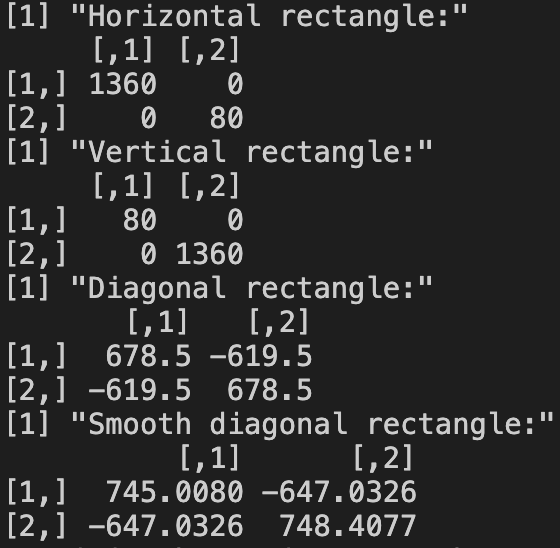
\includegraphics[height=5cm]{rectangles-moments.png}
    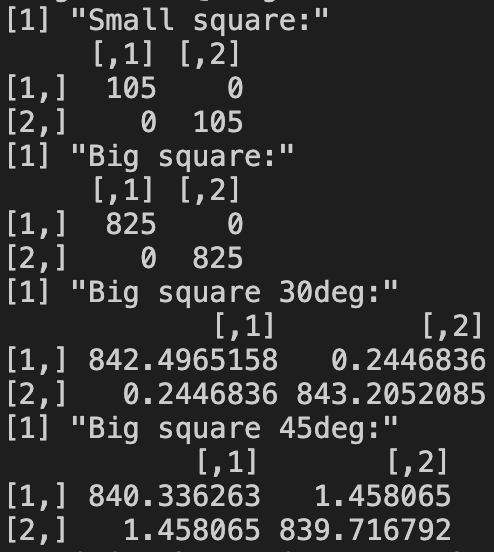
\includegraphics[height=5cm]{squares-moments.png}
    \caption{Inertia matrices for rectangles and squares}
\end{figure}
\paragraph{}
Upon calculating the values for the rectangles, we can observe that their matrix of inertia is different for each shape.
For the horizontal rectangle, it's intuitive that the following equation should happen: $\mu_{20} > \mu_{02}$.
That's because there are more pixels distributed over the $x$ axis. For the vertical rectangle, it's the opposite.
The inertia matrix tells us just that.
For the diagonal rectangle, there's an interesting observation: $\mu_{20} = \mu_{02}$. That's because the rectangle is rotated at 45 degrees, so the pixels are uniformely distributed horizontally and vertically.
For the two diagonal rectangles, the surface differs, but it's interesting to notice that the proportion $\frac{\mu_{20}}{\mu_{02}}$ is about the same. That would mean that the rectangles are similarly oriented, which is true.
\paragraph{}
The $\frac{\mu_{20}}{\mu_{02}}$ proportion is also kept in the case of the the squares which aren't rotated.
Another interesting observation is that for the shapes that aren't rotated, $\mu_{11} = 0$.
All of these already give us valuable information as to how the shape looks, so they can definitely be used as shape attributes.
However, we can still improve these.
% -----------------------------------------------

\section{Shape's main axis of inertia}
\subsection{Normalised Moment Centers}
\paragraph{}
For our next trick, we can make $\mu_{ij}$ invariant to the scale of the image. We define the \emph{normalized centered moment} as the following:
$$\eta_{ij} = \frac{\mu_{ij}}{\mu_{00}^{1 + \frac{i + j}{2}}}$$

\begin{lstlisting}[language=R, caption=Calculating normalised centered moments]
    rdfMomentCentreNormalise <- function (img, p, q){
        upq = rdfMomentCentre(img, p, q)
        u00 = rdfMomentCentre(img, 0, 0)
        normalised = upq / (u00 ** (1 + (p + q)/2))
        normalised
    }
\end{lstlisting}

\paragraph{}
Taking a look at $\eta{20}, \eta{02}$ and $\eta{22}$

\begin{figure}[h]
    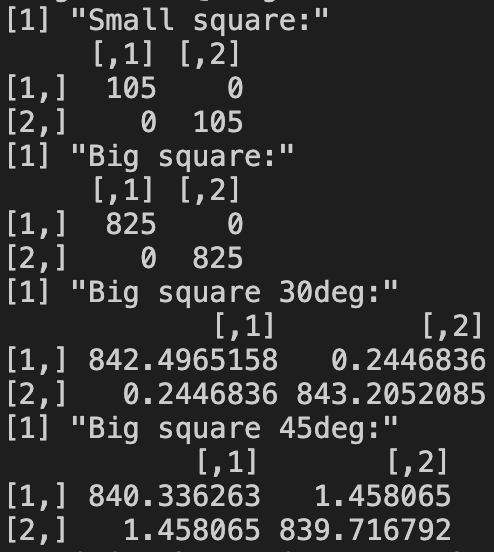
\includegraphics[height=5cm]{squares-moments.png}
    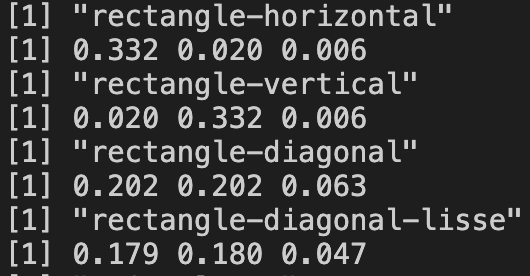
\includegraphics[height=5cm]{rectangles_normalised_moments.png}
    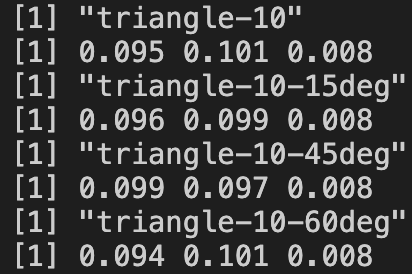
\includegraphics[height=5cm]{triangles_normalised_moments.png}
    \caption{Normalised moment centers}
\end{figure}

% \subsection{Main axis of inertia}
% \paragraph{}
% Inspiring ourselves from physics, we may use the shape's moment of inertia matrix. With that, we're able to tell which is a figure's main axis of inertia.

% \begin{lstlisting}[language=Python, caption=Calculating normalised centered moments]
% def mainInertionAxis(img, normalise=True):
%     f = rdfMomentCentreNormalise if normalise is True else rdfMomentCentre
%     u20 = f(img, 2, 0)
%     u11 = f(img, 1, 1)
%     u02 = f(img, 0, 2)
%     I = np.ndarray(buffer=np.array(
%         [u20, u11, u11, u02]), shape=(2, 2), dtype='float')
%     _, eigenVectors = np.linalg.eig(I)
%     P = eigenVectors.T
%     return P
% \end{lstlisting}

% \paragraph{}
% Our first experiment is calculating the main axis for the 3 rectangles, in the following order: diagonal, horizontal and vertical. The results clearly show us that we can easily differentiate the fact that the shapes are rotated.
% \begin{figure}[h]
%     \centering
%     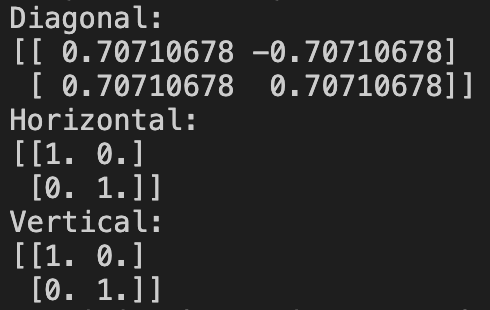
\includegraphics{main_axis_rectangles.png}
%     \label{fig:main-axis-rectangles}
% \end{figure}

% \paragraph{}
% Let us now analyse the square images. From the results, we can see that the main axis of inertia for the squares that only differ in size is the same.
% For the square that is rotated, we get different results. Therefore, calculating the main axis of inertia is invariant to the scale of the shape.
% \begin{figure}[h]
%     \centering
%     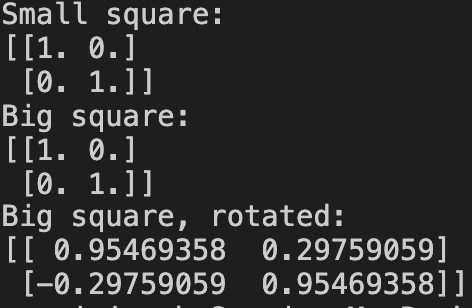
\includegraphics{main_axis_squares.png}
%     \label{fig:main-axis-squares}
% \end{figure}

% % \begin{figure}
% %     \begin{subfigure}
% %         \centering
% %         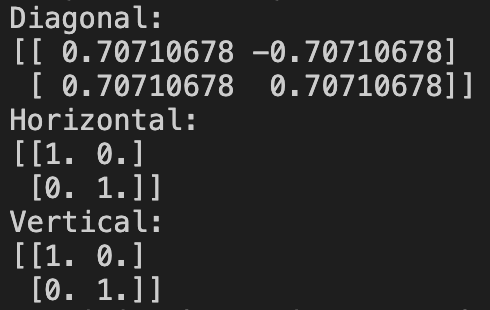
\includegraphics{main_axis_rectangles.png}
% %         \label{fig:main-axis-rectangles}
% %     \end{subfigure}

% %     \begin{subfigure}
% %         \centering
% %         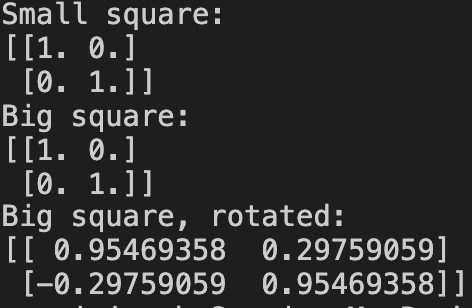
\includegraphics{main_axis_squares.png}
% %         \label{fig:main-axis-squares}
% %     \end{subfigure}
% % \end{figure}